% File: ot.tex


\documentclass{standalone}

\usepackage{tikz}
\usetikzlibrary{shapes, positioning, arrows.meta, calc, intersections, backgrounds, fit}

% default horizontal/vertical distance
\def\hdist{1.5}
\def\vdist{1.5}
\tikzset{node distance = \vdist and \hdist}

\newcommand{\state}[3]{% #1: state name; #2: position; #3: state label
  \node (#1) [circle, inner sep = 0pt, minimum size = 8mm, text width = 8mm, align = center, draw, #2, font = \Large] {#3};
}

\newcommand{\trans}[5]{% #1: start state; #2: end state; #3: transition label; #4: transition label position; #5: style
  \draw[>=Stealth, ->,  #5] (#1) to node [rectangle, draw, above = 2pt, sloped, #4] {#3} (#2);
}

\begin{document}
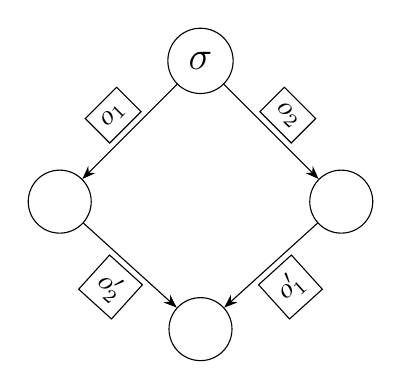
\begin{tikzpicture}
  \state{0}{}{$\sigma$}
  \state{l}{below left = of 0.center}{}
  \state{r}{below right = of 0.center}{}
  \state{lr}{below = 2*\vdist of 0.center}{}

  \trans{0}{l}{$o_1$}{}{}
  \trans{0}{r}{$o_2$}{}{}
  \trans{l}{lr}{$o'_2$}{below = 2pt}{}
  \trans{r}{lr}{$o'_1$}{below = 2pt}{}
\end{tikzpicture}
\end{document}
